
\section*{Eidesstattliche Erklärung}
Hiermit erkläre ich an Eides statt, dass ich die vorgelegte Diplomarbeit selbstständig und ohne Benutzung anderer als der angegebenen Hilfsmittel angefertigt habe. Gedanken, die aus fremden Quellen direkt oder indirekt übernommen wurden, sind als solche gekennzeichnet.

Die Arbeit wurde bisher in gleicher oder ähnlicher Weise keiner anderen Prüfungsbehörde vorgelegt und auch noch nicht veröffentlicht. \\[1em]
Leonding, am \duedatede \\[5em]
\ifthenelse{\isundefined{\firstauthor}}{}{\firstauthor}
\ifthenelse{\isundefined{\secondauthor}}{}{\kern-1ex, \secondauthor}
\ifthenelse{\isundefined{\thirdauthor}}{}{\kern-1ex, \thirdauthor} \\[5em]


\begin{abstract}
\underline{Aufgabenstellung}:
Für das Unternehmen Augenoptik Aigner in Wels ist ein Verwaltungsprogramm und eine neue Website zu gestalten. \newline Die Website ist responsive zu entwickeln. Auf dieser sollen neben der Lage und den Öffnungszeiten auch die verschiedenen Brillenmodelle angezeigt werden. Der User kann über die Website dem Verkäufer sein Kaufinteresse mitteilen. Der Verkäufer kann sich auf der Website anmelden und, dann seine Tabellen ansehen und bearbeiten um zum Beispiel von zu Hause eine neue Brille einzutragen. \newline Die Website soll für Kunden ansprechend sein und eine gute Übersicht über die Brillenmodelle bieten außerdem sollte der Administrator der Website die Möglichkeit haben von zu Hause seine Brillenmodelle zu verwalten. 
\newline Für die Verwaltungssoftware ist eine Desktopanwendung zu entwickeln, die das bisher verwendete Programm vollständig ersetzen soll. Die Software soll auf mehreren Rechnern synchronisiert verwendbar sein und alle  Kunden, Aufträge, Lieferanten und Brillenfassungen verwalten. Zusätzlich sollen aus dem Programm Word-Dokumente exportiert werden können (z.B. Rechnungen) und der Benutzer soll eine Statistik über seine verkauften Brillen und Kontaktlinsen sehen. Außerdem soll es möglich sein aus dem Programm heraus E-Mails und SMS zu versenden. \newline
\underline{Realisierung}:
Die aktuelle Website ist nicht mobile responsive und sie der einzigen Funktionen sind den Verkäufer zu kontaktieren und allgemeine Daten anzusehen.
Die Website hätte man in verschiedenn Programmiersprachen umsetzen können.
Sie wurde aufgrund der Vorkenntnisse mittels Asp .net entwickelt. Es wurde das Mvc-Pattern umgesetzt. \newline Das aktuell verwendete Verwaltungssystem ist ein veraltetes Microsoft DOS-Programm, welches umständlich und zeitaufwendig zu bedienen ist. Zur Realisierung der neuen Version wurde WPF mit dem MVVM-Pattern (angewandt mit MVVM-Light) verwendet. Der Zugriff auf die Datenbank wurde mittels dem Entity-Framework und dem UnitOfWork-Pattern realisiert.
\newline \underline{Ergebnisse:} Es ist eine fertige mobile responsvie Website die dem Unternehmen Augenoptik Aigner zur Verfügung gestellt wird. \newline Das Ergebnis des Verwaltungsprogrammes ist ein fertiges Softwareprodukt, das demnächst im Unternehmen Augenoptik Aigner eingesetzt werden soll. Die Software kann in der beigelegten CD begutachtet werden.
\begin{figure}
	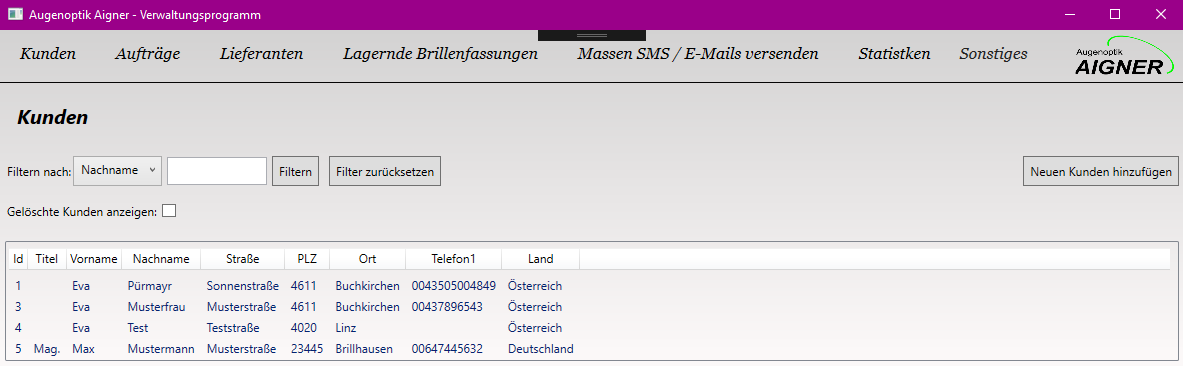
\includegraphics[scale=0.47]{images/abstract.png}
	\caption{Screenshot des Verwaltungsprogrammes}
	\label{fig:sample}
\end{figure}
\end{abstract}
\begin{otherlanguage}{english}
\begin{abstract}

\end{abstract}
\end{otherlanguage}
\newpage \newpage
\section*{Danksagung}
An dieser Stelle möchten wir unserem Betreuungslehrer Herrn Professor Bucek für die sehr strukturierte und engagierte Betreuung der Diplomarbeit danken. Besonders tatkräftig hat er uns geholfen, wenn es wiedereinmal um unerklärliche Programmierprobleme ging. \newline Außerdem möchten wir uns bei unserem Auftraggeber Herrn Wolfgang Aigner für die interessante Aufgabenstellung bedanken. Zusätzlich schätzen wir die Zeit, die er für unsere Fragen aufgebracht hat.
